\section{Method}

This section outlines our method which consist of two sub-sections: the model and the training routine. The model sub-section details the structure of our proposed error correction system which is split into two parts, the error detection stage and the error correction stage. The training routine describes the data augmentation techniques found effective for each of the datasets the model was applied to.

\subsection{Model}

Two variants of the model is discussed in this paper, with the major different being the token the model operates on: word tokens, and SentencPiece tokens. Minor differences are detailed in the corresponding subsections. The model is splitted into two stages: the error detection stage and the error correction stage. The error detection stage, given an input of a sequence of tokens which contains erroneous text \(\vec{t} = \{t_{1}, t_{2}, \dots, t_{N}\}\), predicts a sequence of label \(\vec{l} = \{l_{1}, l_{2}, \dots, l_{N}\}\). Where \(N\) is the number of tokens and the \(l_{i}\) denote the label predicted by the model for the corresponding token \(t_{i}\). A token can be labeled as either correct, or erroneous \(l_{i} \in \{error, correct\}\). Where the model should label the tokens as an error \(l_i = error\) if the token requires correction or label the tokens as a correct token \(l_i = correct\) if the tokens does not require correction.

While the error correction stage is given the same sequence of tokens containing erroneous text and the prediction from the error detection model. The error correction model produces a new sequence \(\vec{t^*} = \{t^*_{1}, t^*_{2}, \dots, t^*_{M}\}\) where every token \(t_i\) marked as correct \(l_i = correct\) is left unaltered \(t_i \in \vec{t^*}\) where \(l_i = correct\).

\subsubsection{Error Detection}

Our proposed error detection model is a standard Bi-LSTM-based sequence tagger, an illustration is shown in Fig~\ref{fig:detection-model}. The model consist of word embedding layer, an optional character embedding layer, 2 layer bidirectional LSTM, and a output dense projection layer with a softmax activation function. The character-level embeddings are obtained by encoding each character of a token into a single vector using another character Bi-LSTM, an illustration is shown in Fig~\ref{fig:char-lstm-encoder}. Character-embeddings are only used for modeling errors detector on word tokenized sequences, as models based on word tokens suffer from out-of-vocabulary (OOV) tokens. For our model variant which uses SentencePiece tokenization, OOV is not an issue, thus only the token embeddings are present. Experiments conducted during hyper-parameter tuning confirms that the inclusion of character-embeddings with SentencePiece results in worse generalization, which is likely due to overfitting.

\begin{figure}
    \centering
    \begin{subfigure}{.5\textwidth}
        \centering
        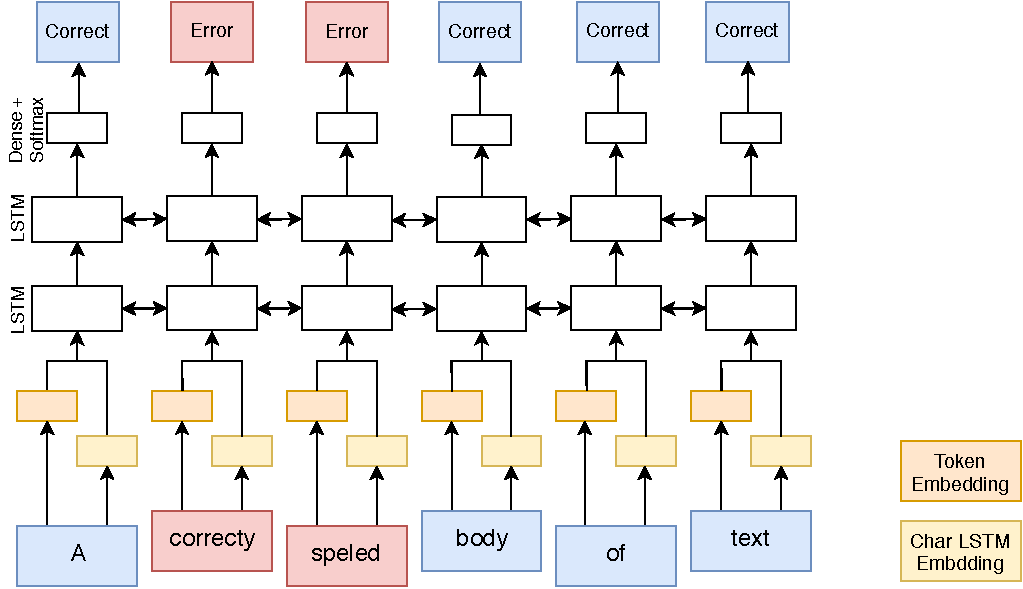
\includegraphics[width=.8\linewidth]{diagrams/detection-model.pdf}
        \caption{Error detection on a sequence.}
        \label{fig:detection-model-struct}
    \end{subfigure}%
    \begin{subfigure}{.5\textwidth}
        \centering
        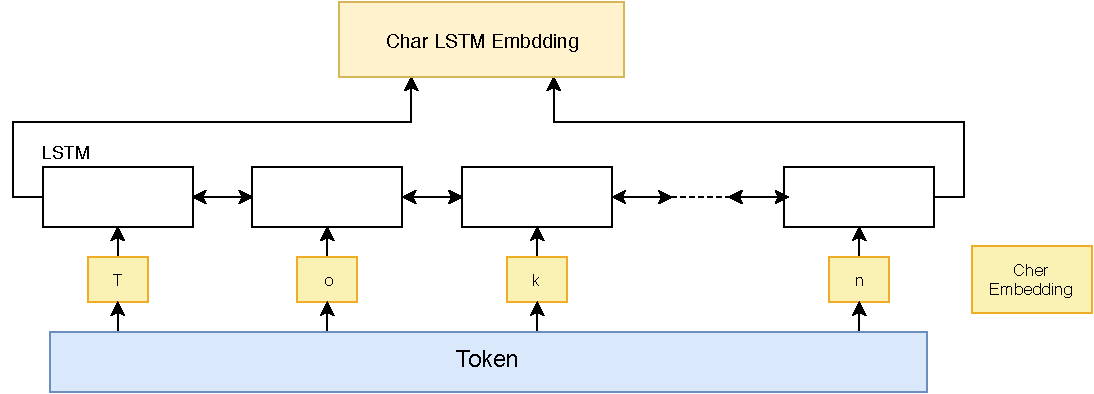
\includegraphics[width=.8\linewidth]{diagrams/char-lstm-encoder.pdf}
        \caption{Char LSTM embedding encoding a token.}
        \label{fig:char-lstm-encoder}
    \end{subfigure}
    \caption{Error detection model}
    \label{fig:detection-model}
\end{figure}

\subsubsection{Error Correction}

Our proposed error correction model is a sequence-to-sequence network given a sequence of erroneous input characters predicts a sequence of tokens corresponding to the correction of the input while also take into account the context of the sequence. Our model is structured as a sequence-to-sequence (Seq2Seq) network which can be grouped into 2 parts, the encoder and the decoder. An illustration of the overall structure is shown in Fig~\ref{fig:correction-model-struct}. The encoder features a novel use of the bidirectional attention flow network (BiDAF) [ref] to encode both the error sequence and the context sequence into a sequence of embeddings. The BiDAF network is a substitution to a typical embedding layer in a Seq2Seq encoder. BiDAF is a proven achitecure was originally designed to model 2 text sequences for the Machine Comprehension task. The structure of BiDAF network allows the model to embed information from the context sequence into the error sequence allowing our network to model from both the error sequences and the context sequence.

\begin{figure}
    \centering
    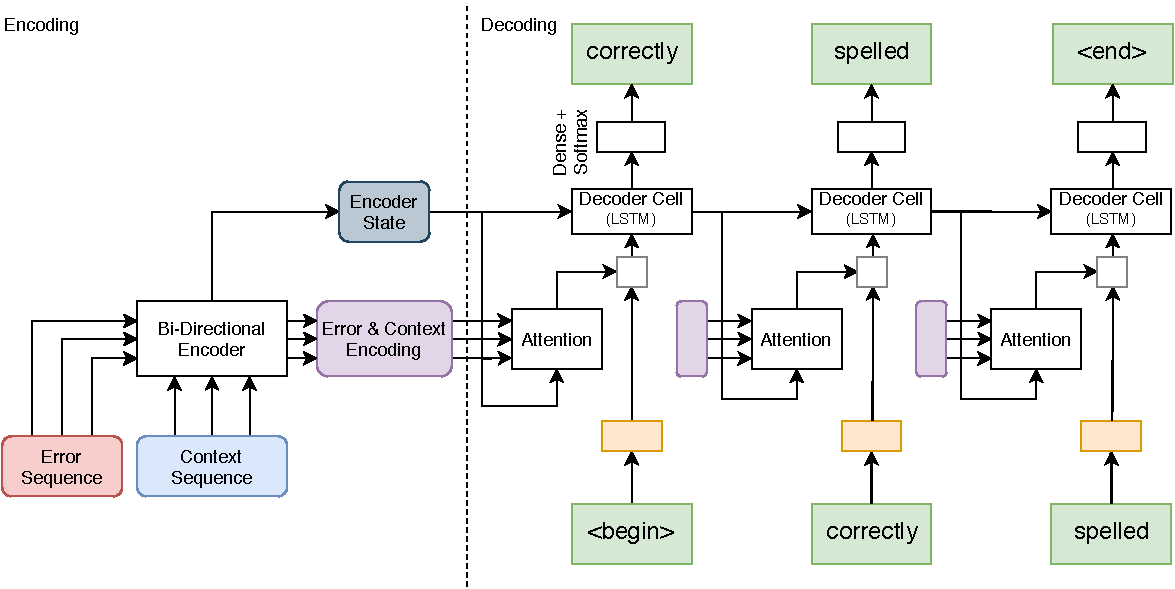
\includegraphics[width=.8\linewidth]{diagrams/correction-seq2seq-model.pdf}
    \caption{Structure of the proposed error correction Seq2Seq model. The model can be viewed as two separated parts: the encoder and decoder, denoted by the dotted line. This figure highlights the decoder, a detailed view of the encoder is shown in Fig~\ref{fig:bidaf-encoder}. Three parallel arrows represent passing a sequence of vectors while a single arrow represent a single vector. White box without a label represents a concatenation operation. Orange box represents an token embedding layer.}
    \label{fig:correction-model-struct}
    \centering
    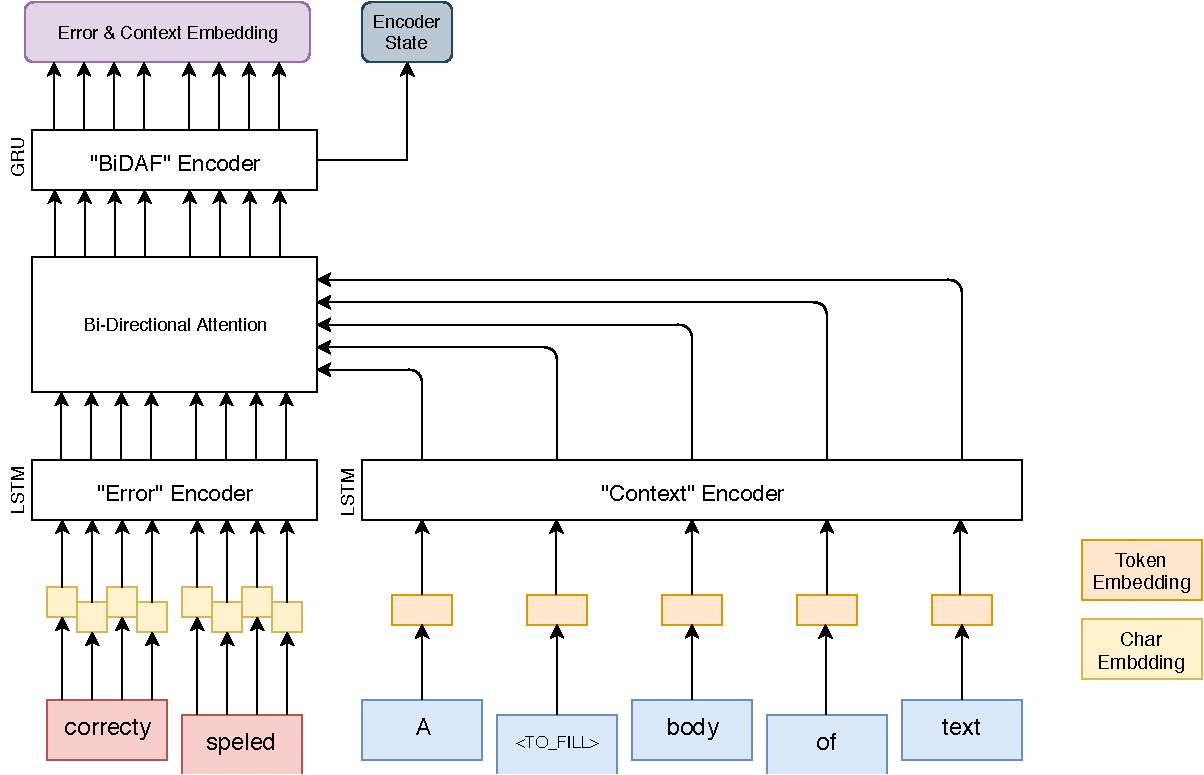
\includegraphics[width=.8\linewidth]{diagrams/bidaf-encoder.pdf}
    \caption{Bi-directional encoder encoding an error segment along side its context. All LSTM boxes and GRUx2 boxes each represent a bidirectional recurrent layer. The "<TO\_FILL>" token represents a special token denoting the position of the erroneous input within the context. Note that both the error input and context also feature a special "<BEGIN>" and "<END>" token but is omitted to reduce clutter.}
    \label{fig:bidaf-encoder}
\end{figure}

\subsubsection*{BiDAF encoder}
The structure of the BiDAF encoder is shown in Fig~\ref{fig:bidaf-encoder}. [TODO]

\subsubsection*{Decoder}
The decoder is a standard LSTM decoder with attention mechanism for observing the BiDAF encoded sequence, an illustration is shown in Fig~\ref{fig:correction-model-struct}.

\subsection{Training}
